This layer involves the various sensors and indicators that interact between the Turing Board and the user. This includes the weight sensor used to detect if the rider falls off the board, triggering an emergency stop. It also detects if the user attempts to step on the board during autonomous mode. This, in turn, would trigger a speaker/buzzer to beep until the board finishes rotating the front turning mechanism back to neutral and locks it in place. An anklet will be used to help the Turing Board find the rider and track them when in follow-along mode. These are all interconnected with the central control unit and the various modes being implemented in the final product. As a result, we are implementing an LED strip to help indicate to the user what mode the Turing Board is currently in, specified by different color lights.

\subsection{Pressure Sensor}
The pressure sensor will be implemented as a safety feature primarily, with future uses in load carrying. When a user is riding on the board, it will detect if they fall off to initiate an emergency stop. When a user attempts to get on the board while in autonomous mode it will trigger an alert noise to notify the user it is not safe to ride.

\begin{figure}[h!]
	\centering
 	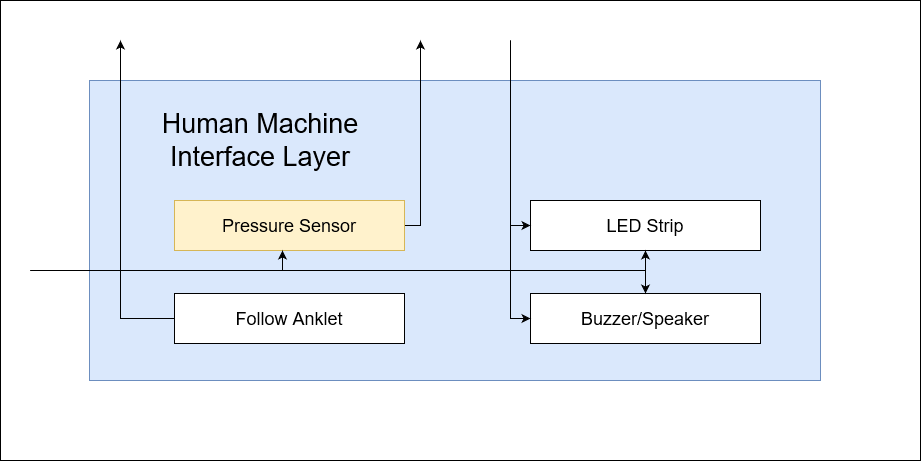
\includegraphics[width=0.60\textwidth]{ADS Latex/images/Kendall/Pressure Sensor.png}
 \caption{Pressure Sensor}
\end{figure}

\subsubsection{Assumptions}
This subsystem is assumed to interact with the Jetson TX2 to send a signal to the motorized wheels and turning mechanism and the buzzer/speaker. It will be activated nearly all the time to detect when a rider has fallen off or attempts to get on, both in autonomous or riding mode.

\subsubsection{Responsibilities}
The pressure sensor is responsible for alerting the Jetson TX2 when a rider has either stood on or fallen off the Turing Board. In the event the rider falls off, the pressure sensor will signal for an emergency stop. In the event the rider stands on the board when in autonomous mode, it will signal for an emergency buzzer to alert the rider it is not safe to stand on the board yet.

\subsubsection{Subsystem Interfaces}
Each of the inputs and outputs for the subsystem are defined here.

\begin {table}[H]
\caption {Subsystem interfaces} 
\begin{center}
    \begin{tabular}{ | p{1cm} | p{6cm} | p{3cm} | p{3cm} |}
    \hline
    ID & Description & Inputs & Outputs \\ \hline
    \#xx & Connection to Power Subsystem & \pbox{3cm}{Power} & \pbox{3cm}{N/A}  \\ \hline
    \#xx & Connection to Jetson TX2 & \pbox{3cm}{N/A} & \pbox{3cm}{Weight Value}  \\ \hline
    \end{tabular}
\end{center}
\end{table}

\subsection{Buzzer/Speaker}
The buzzer/speaker will be used to alert the user if they attempt to step on the board when it is in an autonomous mode. When the pressure sensor detects a person attempt to stand on the board when in autonomous mode, the buzzer will begin to sound an alert to notify the user it is unsafe to stand on it.

\begin{figure}[h!]
	\centering
 	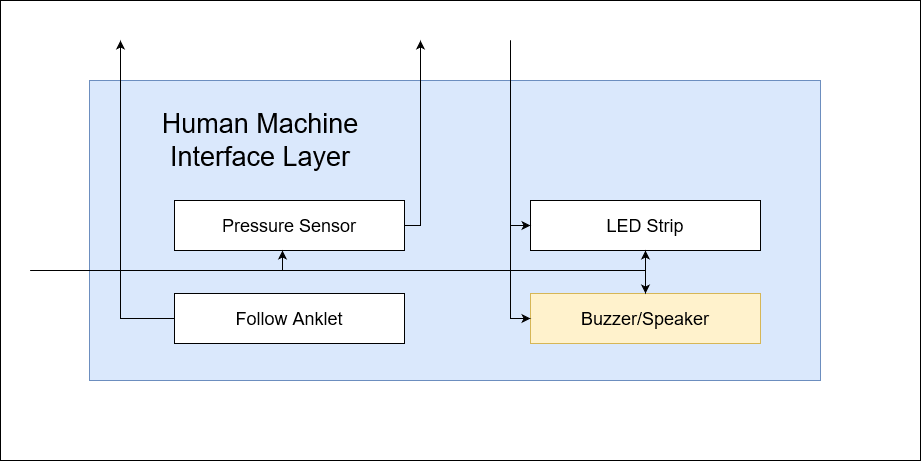
\includegraphics[width=0.60\textwidth]{ADS Latex/images/Kendall/Buzzer.png}
 \caption{Buzzer/Speaker}
\end{figure}

\subsubsection{Assumptions}
This subsystem will receive a signal from the Jetson TX2 to emit a loud noise in the event the pressure sensor detects a weight on the board when not in rider mode. This will only be activated by the Jetson in autonomous mode.

\subsubsection{Responsibilities}
The buzzer/speaker is responsible for alerting the user when it is unsafe to stand on the Turing Board. In the event the rider attempts to stand on the board when in autonomous or follow-along mode, the buzzer will emit a loud noise.

\subsubsection{Subsystem Interfaces}
Each of the inputs and outputs for the subsystem are defined here.

\begin {table}[H]
\caption {Subsystem interfaces} 
\begin{center}
    \begin{tabular}{ | p{1cm} | p{6cm} | p{3cm} | p{3cm} |}
    \hline
    ID & Description & Inputs & Outputs \\ \hline
    \#xx & Connection to Power Subsystem & \pbox{3cm}{Power} & \pbox{3cm}{N/A}  \\ \hline
    \#xx & Connection to Jetson TX2 & \pbox{3cm}{Alert Signal} & \pbox{3cm}{N/A}  \\ \hline
    \end{tabular}
\end{center}
\end{table}

\subsection{LED Strip}
The LED strip will be used to indicate to the user what mode the Turing Board is currently in. These modes will be differentiated by implementing a different color for each mode. 

\begin{figure}[h!]
	\centering
 	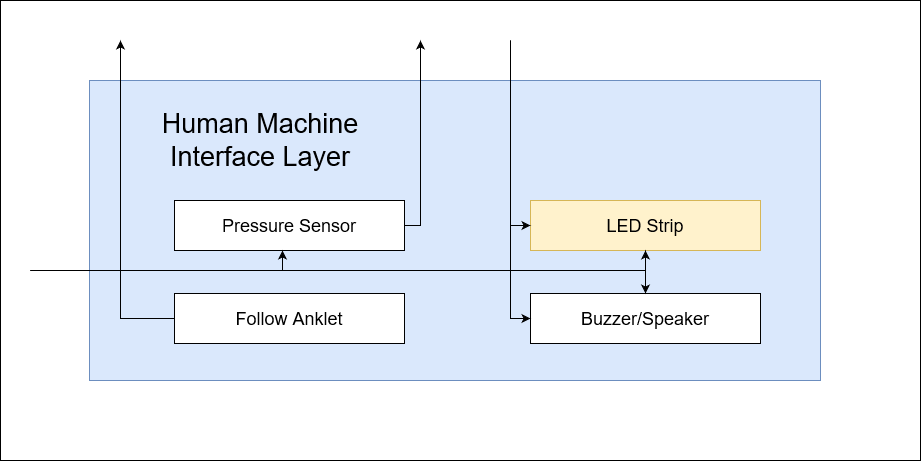
\includegraphics[width=0.60\textwidth]{ADS Latex/images/Kendall/LED Strip.png}
 \caption{LED Strip}
\end{figure}

\subsubsection{Assumptions}
This subsystem will be active most, if not all of the time. It will be able to display different colors to indicate different modes.

\subsubsection{Responsibilities}
The LED strip will be in charge of indicating to the user what mode the Turing Board is currently in. This is done by displaying a different color depending on the mode it is in. It will also be partially responsible for illuminating the area at night.

\subsubsection{Subsystem Interfaces}
Each of the inputs and outputs for the subsystem are defined here.

\begin {table}[H]
\caption {Subsystem interfaces} 
\begin{center}
    \begin{tabular}{ | p{1cm} | p{6cm} | p{3cm} | p{3cm} |}
    \hline
    ID & Description & Inputs & Outputs \\ \hline
    \#xx & Connection to Power Subsystem & \pbox{3cm}{Power} & \pbox{3cm}{N/A}  \\ \hline
    \#xx & Connection to Jetson TX2 & \pbox{3cm}{Mode Indicator Signal} & \pbox{3cm}{N/A}  \\ \hline
    \end{tabular}
\end{center}
\end{table}

\subsection{Follow Anklet}
The Anklet will be a worn feature used for the CV to track and follow the rider in follow-along mode.

\begin{figure}[h!]
	\centering
 	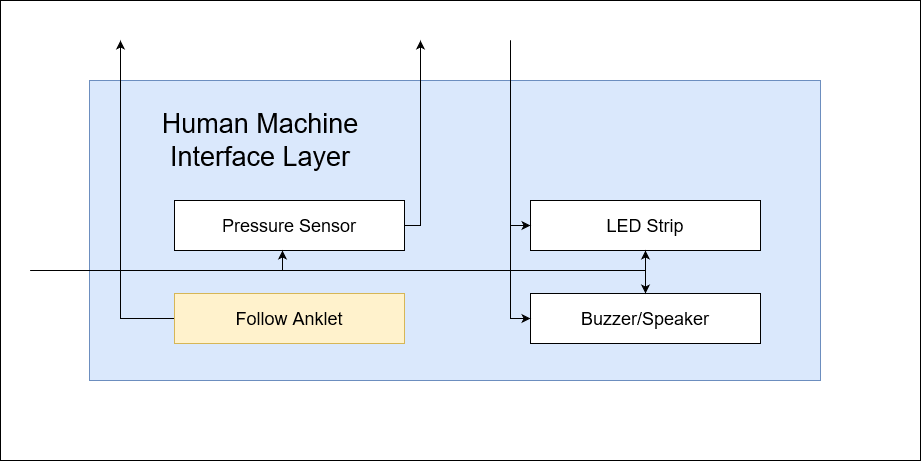
\includegraphics[width=0.60\textwidth]{ADS Latex/images/Kendall/Anklet.png}
 \caption{Follow Anklet}
\end{figure}

\subsubsection{Assumptions}
This subsystem is a worn accessory used to track the user as they walk around. It will only be tracked in follow-along mode. The symbol must be worn around the ankle to be low enough for the camera to see and track it.

\subsubsection{Responsibilities}
The anklet will be responsible for allowing the Turing Board to track the user as they walk around. It will use sensors to track it left and right, adjusting the turning mechanism accordingly to center on it. It will also signal the board to speed up or slow down depending on the distance to the anklet.

\subsubsection{Subsystem Interfaces}
Each of the inputs and outputs for the subsystem are defined here.

\begin {table}[H]
\caption {Subsystem interfaces} 
\begin{center}
    \begin{tabular}{ | p{1cm} | p{6cm} | p{3cm} | p{3cm} |}
    \hline
    ID & Description & Inputs & Outputs \\ \hline
    \#xx & Connection to CV Subsystem & \pbox{3cm}{N/A} & \pbox{3cm}{Tracking Symbol}  \\ \hline
    \end{tabular}
\end{center}
\end{table}

